\documentclass[11pt,a4paper]{article}%
\usepackage{amsmath}
\usepackage{amsfonts}
\usepackage{amssymb}
\usepackage{graphicx}
\usepackage{a4wide}%
\setcounter{MaxMatrixCols}{30}
\usepackage{url}
\usepackage{hyperref}
\usepackage{footnote}
\usepackage{lineno}
\usepackage{pifont}
\usepackage{subfigure} 
\usepackage[subfigure]{tocloft}
\linenumbers
%TCIDATA{OutputFilter=latex2.dll}
%TCIDATA{Version=5.50.0.2960}
%TCIDATA{CSTFile=40 LaTeX article.cst}
%TCIDATA{Created=Friday, April 05, 2013 08:11:12}
%TCIDATA{LastRevised=Tuesday, April 09, 2013 08:44:52}
%TCIDATA{<META NAME="GraphicsSave" CONTENT="32">}
%TCIDATA{<META NAME="SaveForMode" CONTENT="1">}
%TCIDATA{BibliographyScheme=Manual}
%TCIDATA{<META NAME="DocumentShell" CONTENT="Standard LaTeX\Blank - Standard LaTeX Article">}
%BeginMSIPreambleData
\providecommand{\U}[1]{\protect\rule{.1in}{.1in}}
%EndMSIPreambleData
\newtheorem{theorem}{Theorem}
\newtheorem{acknowledgement}[theorem]{Acknowledgement}
\newtheorem{algorithm}[theorem]{Algorithm}
\newtheorem{axiom}[theorem]{Axiom}
\newtheorem{case}[theorem]{Case}
\newtheorem{claim}[theorem]{Claim}
\newtheorem{conclusion}[theorem]{Conclusion}
\newtheorem{condition}[theorem]{Condition}
\newtheorem{conjecture}[theorem]{Conjecture}
\newtheorem{corollary}[theorem]{Corollary}
\newtheorem{criterion}[theorem]{Criterion}
\newtheorem{definition}[theorem]{Definition}
\newtheorem{example}[theorem]{Example}
\newtheorem{exercise}[theorem]{Exercise}
\newtheorem{lemma}[theorem]{Lemma}
\newtheorem{notation}[theorem]{Notation}
\newtheorem{problem}[theorem]{Problem}
\newtheorem{proposition}[theorem]{Proposition}
\newtheorem{remark}[theorem]{Remark}
\newtheorem{solution}[theorem]{Solution}
\newtheorem{summary}[theorem]{Summary}
\newenvironment{proof}[1][Proof]{\noindent\textbf{#1.} }{\ \rule{0.5em}{0.5em}}
\begin{document}

\title{Correlation Time Properties for 1D and 2D Ising Model}
\author{Mateusz Dyndal}
\maketitle

\begin{abstract}
This is short theoretical description of the 
\textbf{IsingTestTCorr.h} test, including the test results.
\end{abstract}

%\newpage

\section{Introduction}
The aim of this project is to simulate the 1D and 2D Ising model using the Monte Carlo algorithms. Interesting properties of the model and the algorithms are observed and presented. Particular attention is given to the correlations in measurement, phase transitions and the determination of the dynamical critical exponent. 
The Ising model considered here is a chain (1D) or square lattice (2D) of spin sites with periodic boundary conditions and the standard Hamiltonian. Spin sites are assigned a value of $s_{i}=\pm1$ to represent spin up/down respectively. Thus, the total magnetization $m$ is the sum of all lattice spin sites:
\begin{equation}
m=\sum_{i}s_{i}
\end{equation}

The Monte Carlo algorithms used for the simulation are: Metropolis and Wolff. 
Metropolis algorithm works by randomly picking a single site on the lattice and flipping it. Wolff, on the other hand, is a cluster-flipping algorithm: it flips a whole growing cluster around a random seed site. 
Care must therefore be taken in defining units of time, as both of these operations occur in one Monte Carlo step. Thus, a single step will refer to a lattice sweep (steps per site) in Metropolis or a single cluster-flip in Wolff algorithm.

In a Metropolis simulation, the successive spin configurations exhibit
a type of critical slowing down near the phase transition temperature
of the finite lattice. This is not the same as relaxation in a real
system. However, it is useful to measure a relaxation time for the
Metropolis dynamics, because it helps to determine how many steps to
skip in order to generate statistically independent configurations.
This means if the correlation time $\tau$ is of the order of a single
Monte Carlo step, then every configuration can be used in measuring
averages. But if the correlation time is longer, then approximately $\tau$ Monte Carlo steps should be discarded between every data point.


\section{Correlation time}
The autocorrelation function for magnetization $\chi(t)$ is defined as:
\begin{equation}
\chi(t) = \int{dt'[m(t')m(t+t')-<m>^2}],
\end{equation}
where $m(t)$ is instantaneous value of magnetization and $<m>$ is its mean value.
From the definition, integration runs from zero to the total time of simulation. 
For practical reasons, the time displacement $t$ takes values from 0 to some predefined $maxTimeseparation$. This time limit can be established in the following way:
$\chi$ values for times $t$ between $maxTimeseparation/2$ and $maxTimeseparation$ oscillate around zero, while for times $t$ less than $maxTimeseparation/2$, exponential decay can be observed. 
Thus, the correlation time $\tau$ can be found by integrating the $\chi(t)$ function:
\begin{equation}
\tau = \int_0^{\infty}{dt~ \dfrac{\chi(t)}{\chi(0)}} \approx \int_0^{maxTimeseparation/2}{dt~ \dfrac{\chi(t)}{\chi(0)}}
\end{equation}
The characteristic time $\tau$ of exponential decay can be also found by fit analysis of 
 $\chi(t)$ as a function of $t$. For Metropolis algorithm and 1D Ising model with $N=2000$ chains and $T=0.5$ such fit is shown on Figure \ref{gt_1d_t05}. Similarly, for $16\times16$ grid of 2D model, this procedure is presented on Figure \ref{gt_2d}.
     

\begin{figure}[!ht]
\centering
  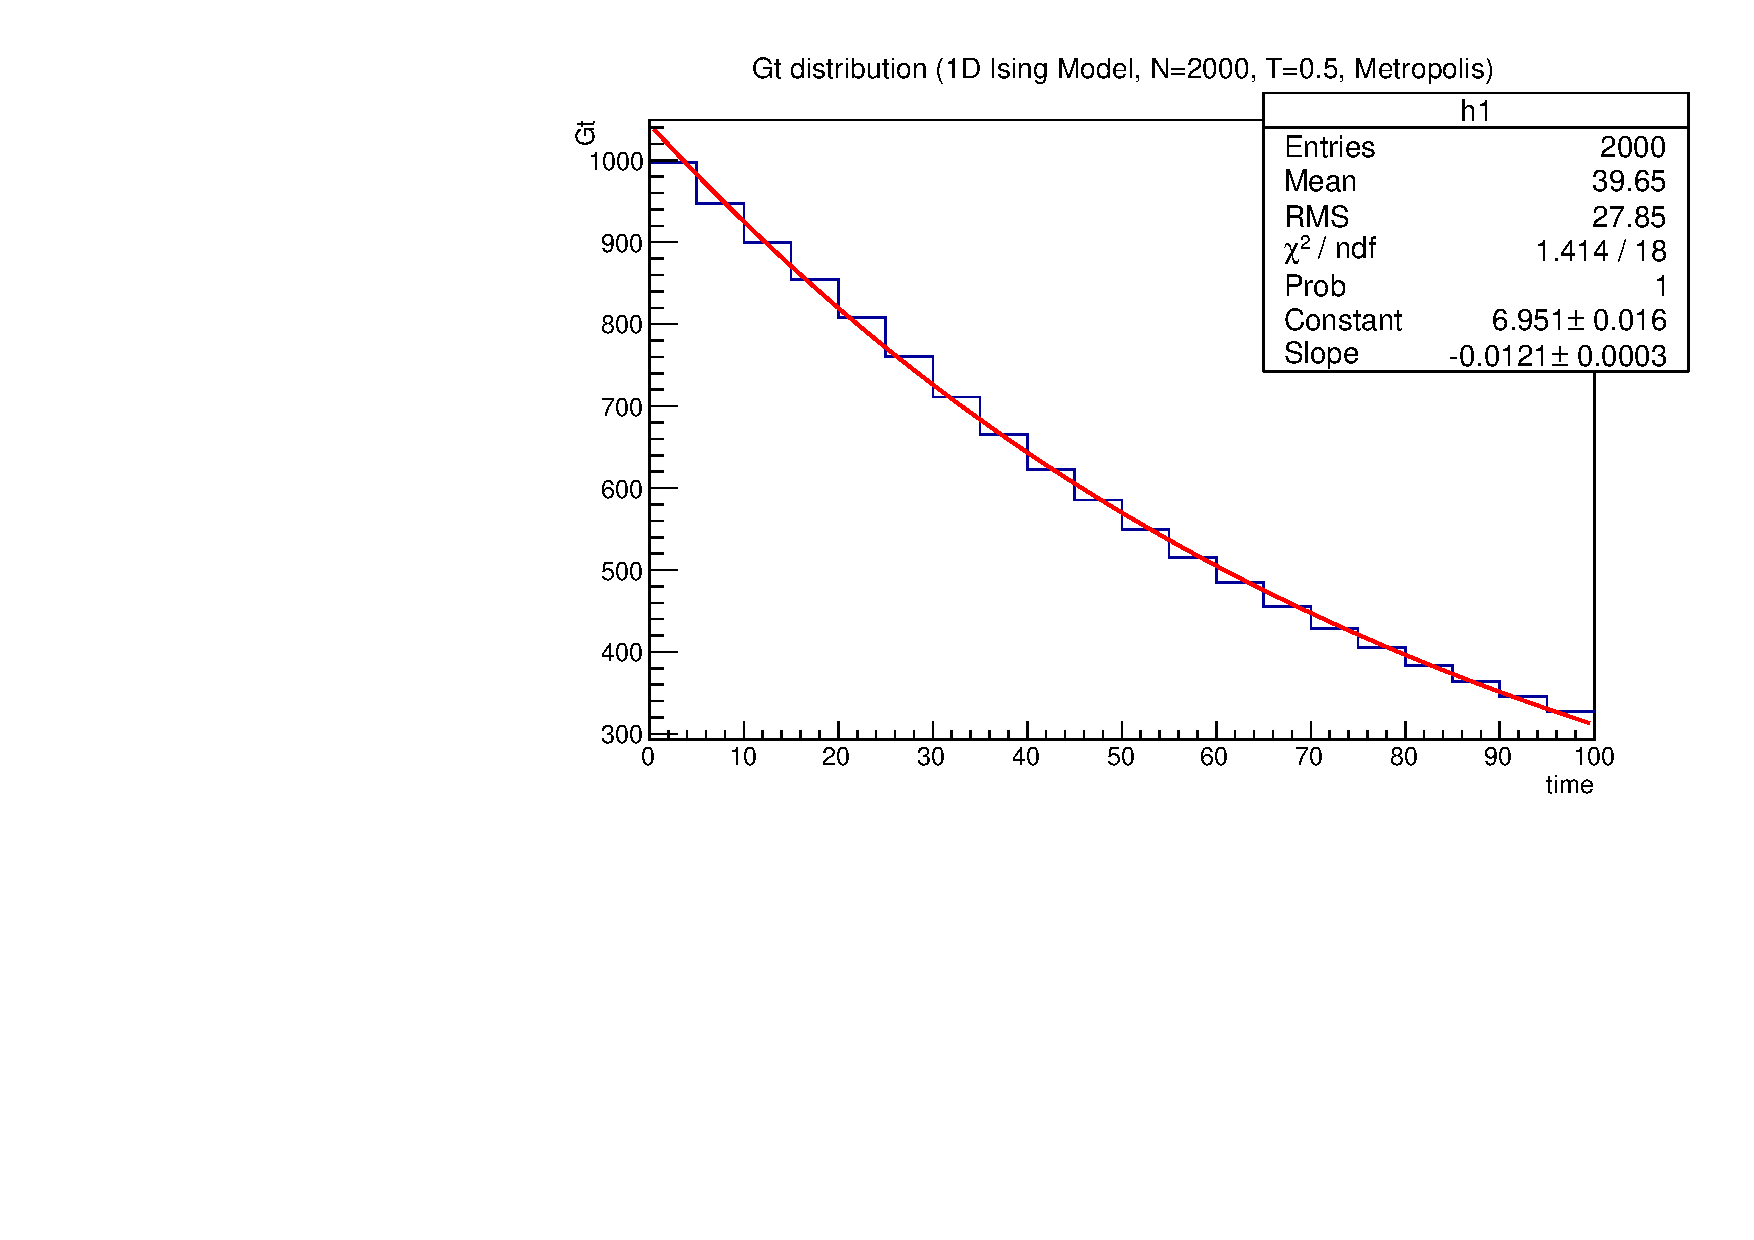
\includegraphics[scale=0.6]{IsingTestTCorr_Gt_1D_T05.pdf}
  \vspace{-0.05in}
   \caption[]{Autocorrelation function (magnetization) for 1D Ising model with $N=2000$ chain of spins and $T=0.5$. The value of the fit slope ($-0.0121$) corresponds to $\tau=82.6$. Metropolis algorithm is used in the simulation.}   
  \label{gt_1d_t05}
\end{figure}



\begin{figure}[!ht]
\centering
  \subfigure{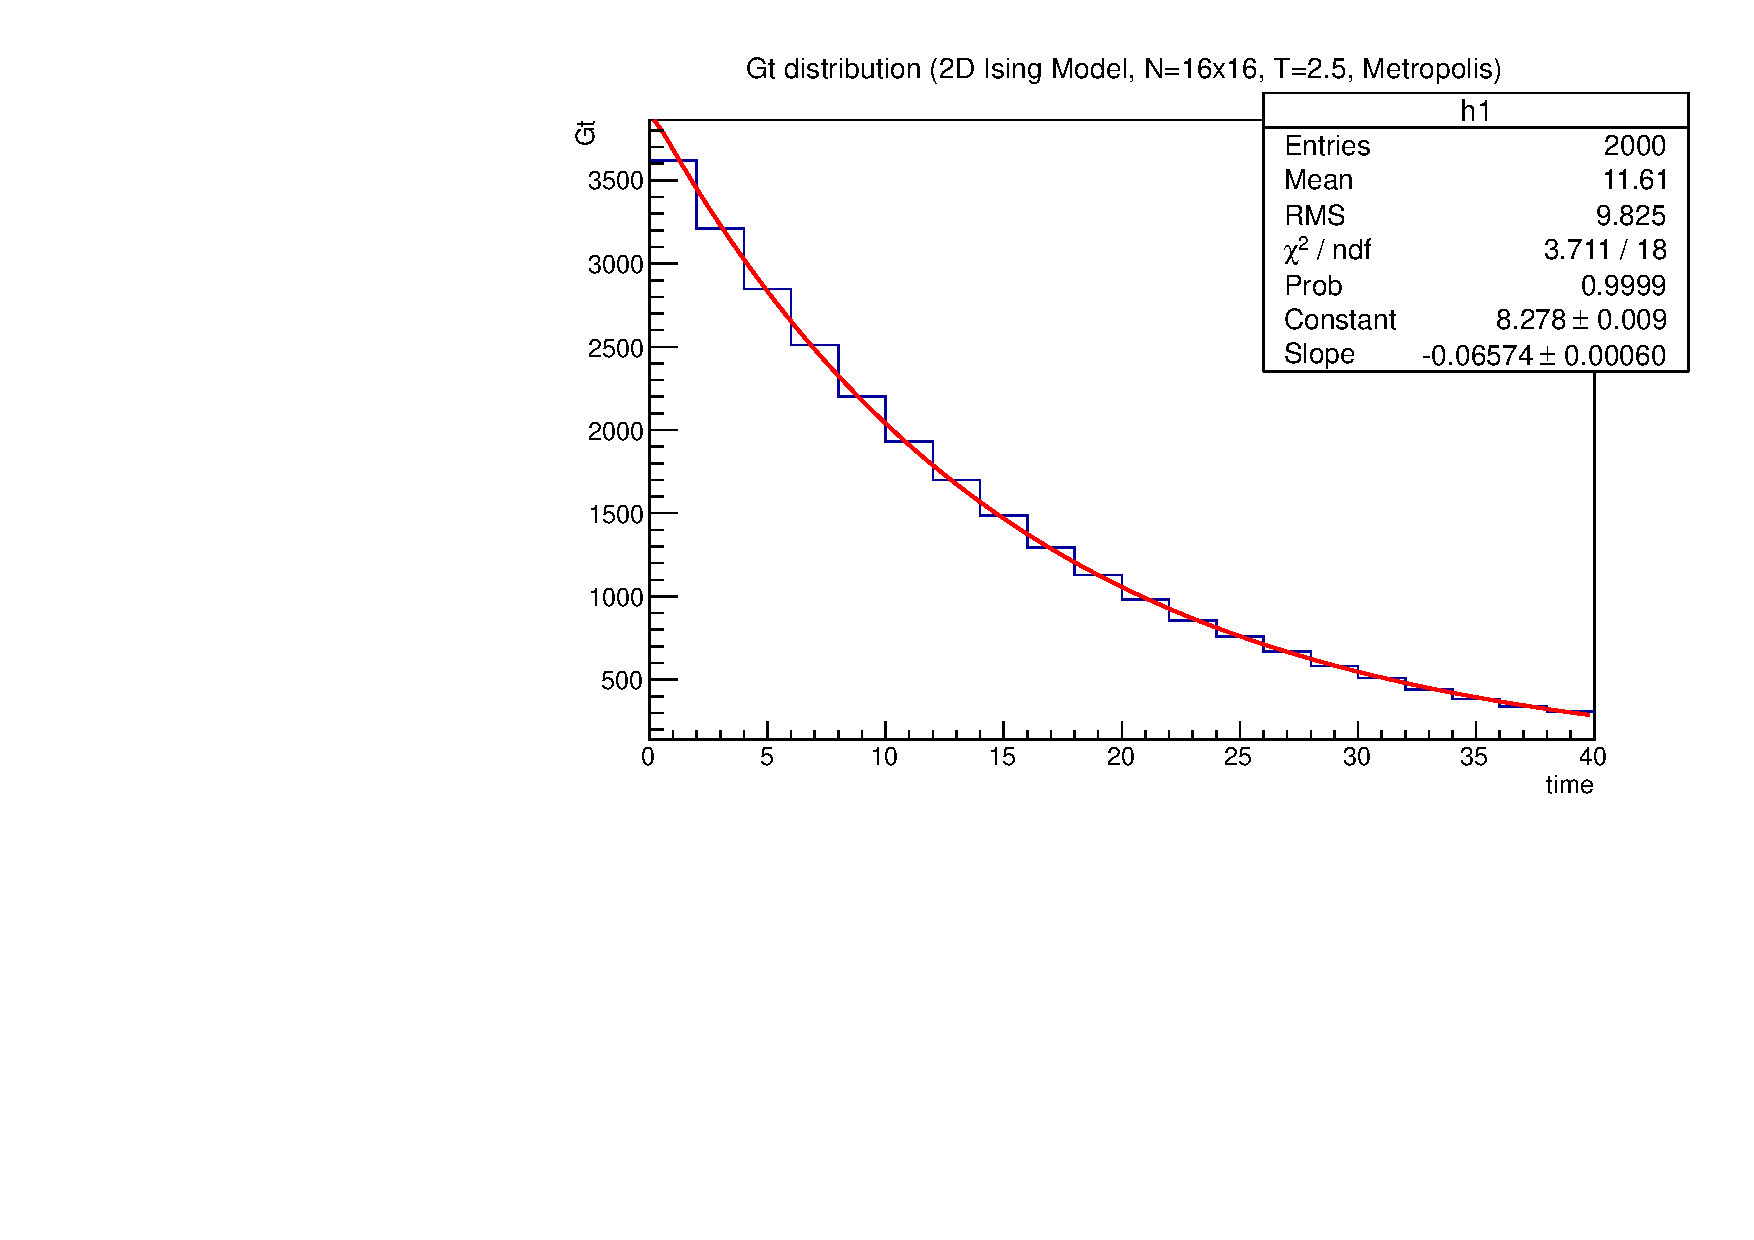
\includegraphics[scale=0.6]{IsingTestTCorr_Gt_2D_T25.pdf}}
  \hspace{-0.15in}
  \subfigure{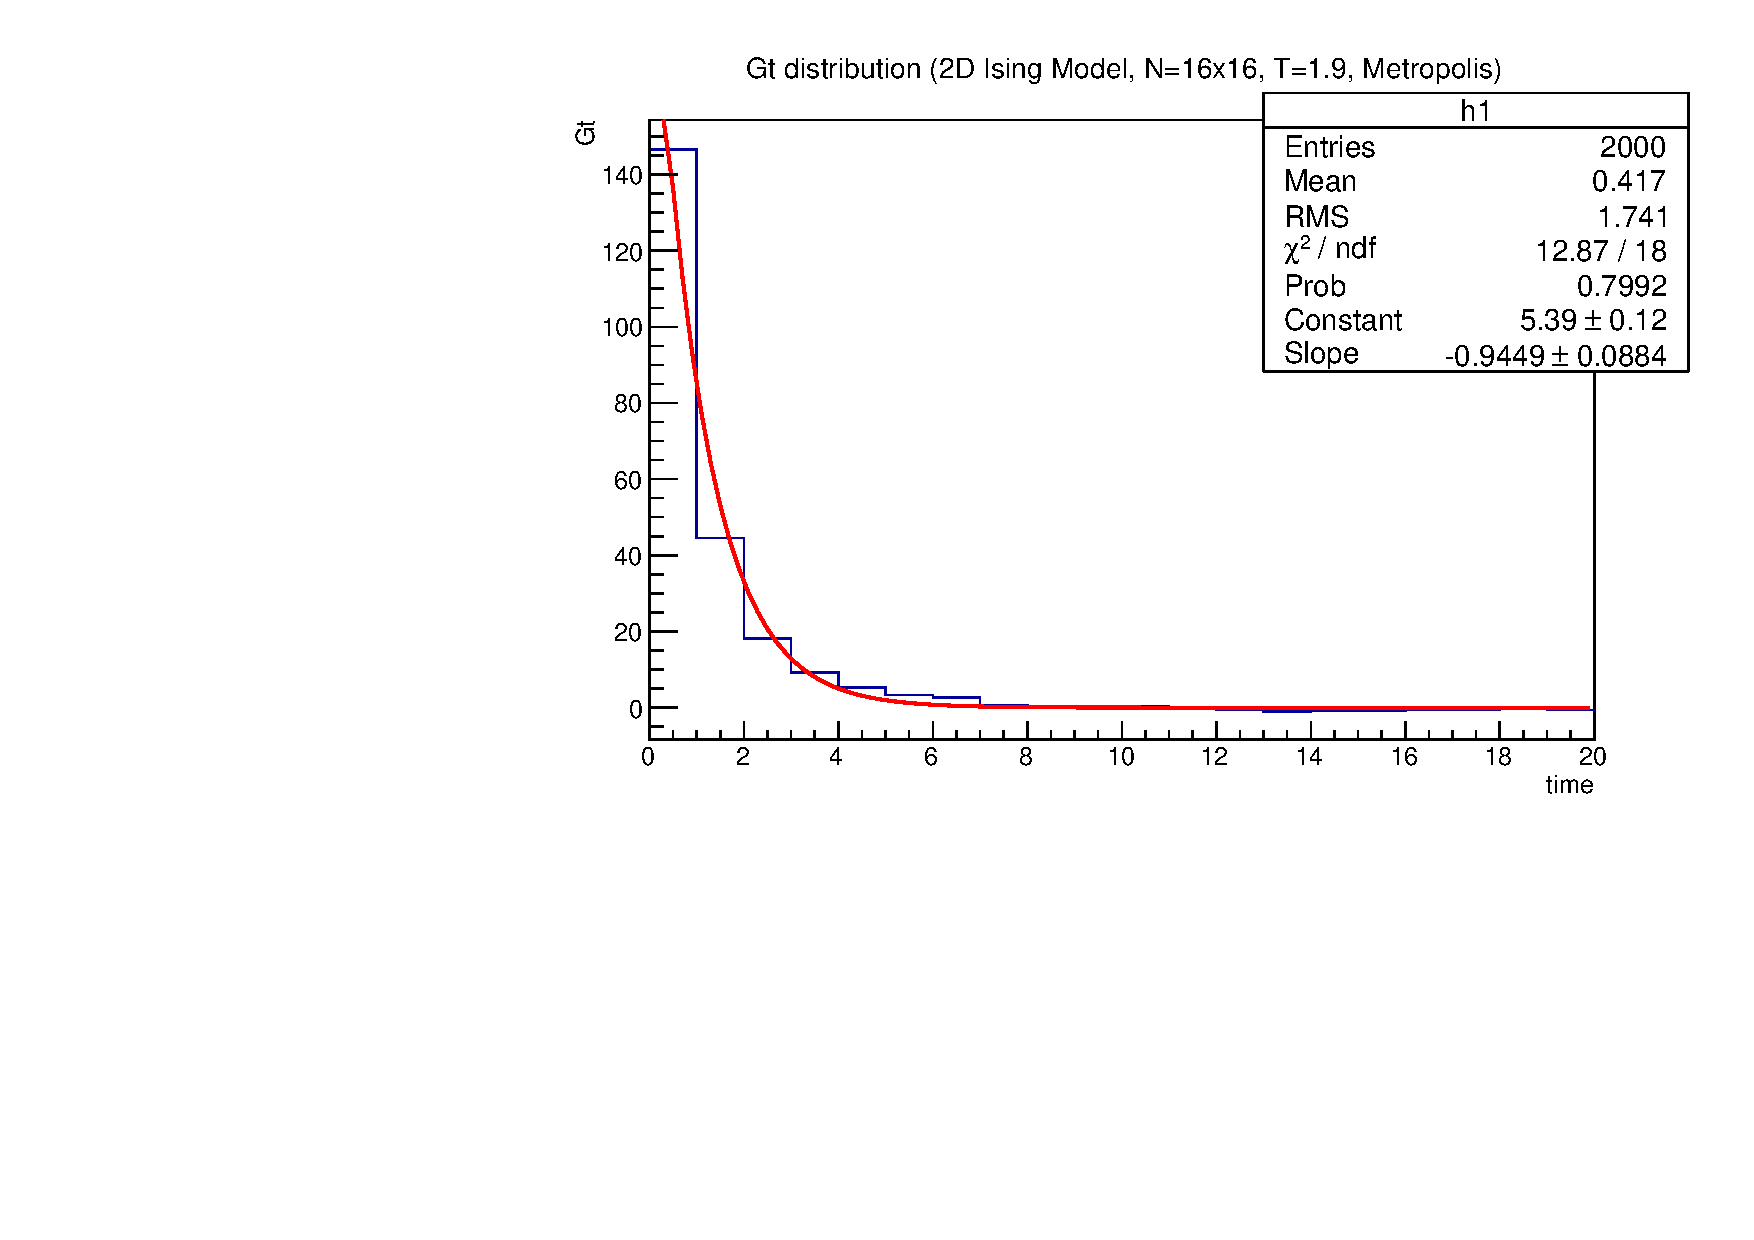
\includegraphics[scale=0.6]{IsingTestTCorr_Gt_2D_T19.pdf}} 
  \vspace{-0.05in}
   \caption[]{(top) Autocorrelation function (magnetization) for 2D Ising model with $N=16\times16$ lattice of spins and $T=2.5$. The value of the fit slope corresponds to $\tau=15.2$.

(bottom) Same but with $T=1.9$ which results in $\tau=1.06$. In both cases Metropolis algorithm is used in the simulation.}   
  \label{gt_2d}
\end{figure}


\clearpage
\section{Relationship with critical exponents}
 The critical exponents of the transition in the Ising model are universal values and characterise the singular properties of physical quantities. In particular, the relaxation time becomes very large near the critical temperature and can be shown to diverge for an infinite system:
\begin{equation}
\tau \sim \xi^z  ,
\label{tauxi}
\end{equation}
or equivalently:
\begin{equation}
\tau \sim t^{-\nu z} .
\label{tauxi2}
\end{equation}
This phenomenon is called critical slowing down. Here $z$ is the dynamical critical exponent associated with a given correlation function, $\xi$ is the correlation length with its critical exponent $\nu$ and $t$ is a reduced temperature, i.e.:
\begin{equation}
t=\dfrac{T-T_c}{T_c} . 
 \end{equation}
Practically, for a finite simulated system, $\xi$ is limited by
the system size $L$, so that $\tau \sim L^z $
at the incipient critical point ($T \approx T_c$). 

This behaviour has a connection with the computer (CPU) time in Monte Carlo techniques, required to obtain a fixed number of statistically independent configurations for a system. It scales with $L$ as:
\begin{equation}
CPU \sim L^{d+z} ,
\end{equation}
where $d$ is a spatial dimension of the simulated model. As an example, dynamical critical exponent $z$ is known to be approximately $2$ using the Metropolis algorithm.

\subsection{1D Ising model}
Figure \ref{T_vs_tau_1d} presents the correlation time behaviour as a function of temperature for 1D Ising model ($N=2000$) with Metropolis dynamics. This shows that correlation time becomes very large when the system is reaching the critical temperature ($T_c \approx 0$ for 1D Ising model).

To get the value of dynamical critical exponent of magnetization for Metropolis algorithm (1D model), one can use the relation (\ref{tauxi}). The correlation time dependence on correlation length is shown on Figure \ref{tauxi}. To get the value of critical exponent $z$, a power function fit is performed. The power parameter from the fit gives the value of $z \approx 1.99$, which is in agreement with the expectations.

\begin{figure}[!ht]
\centering
  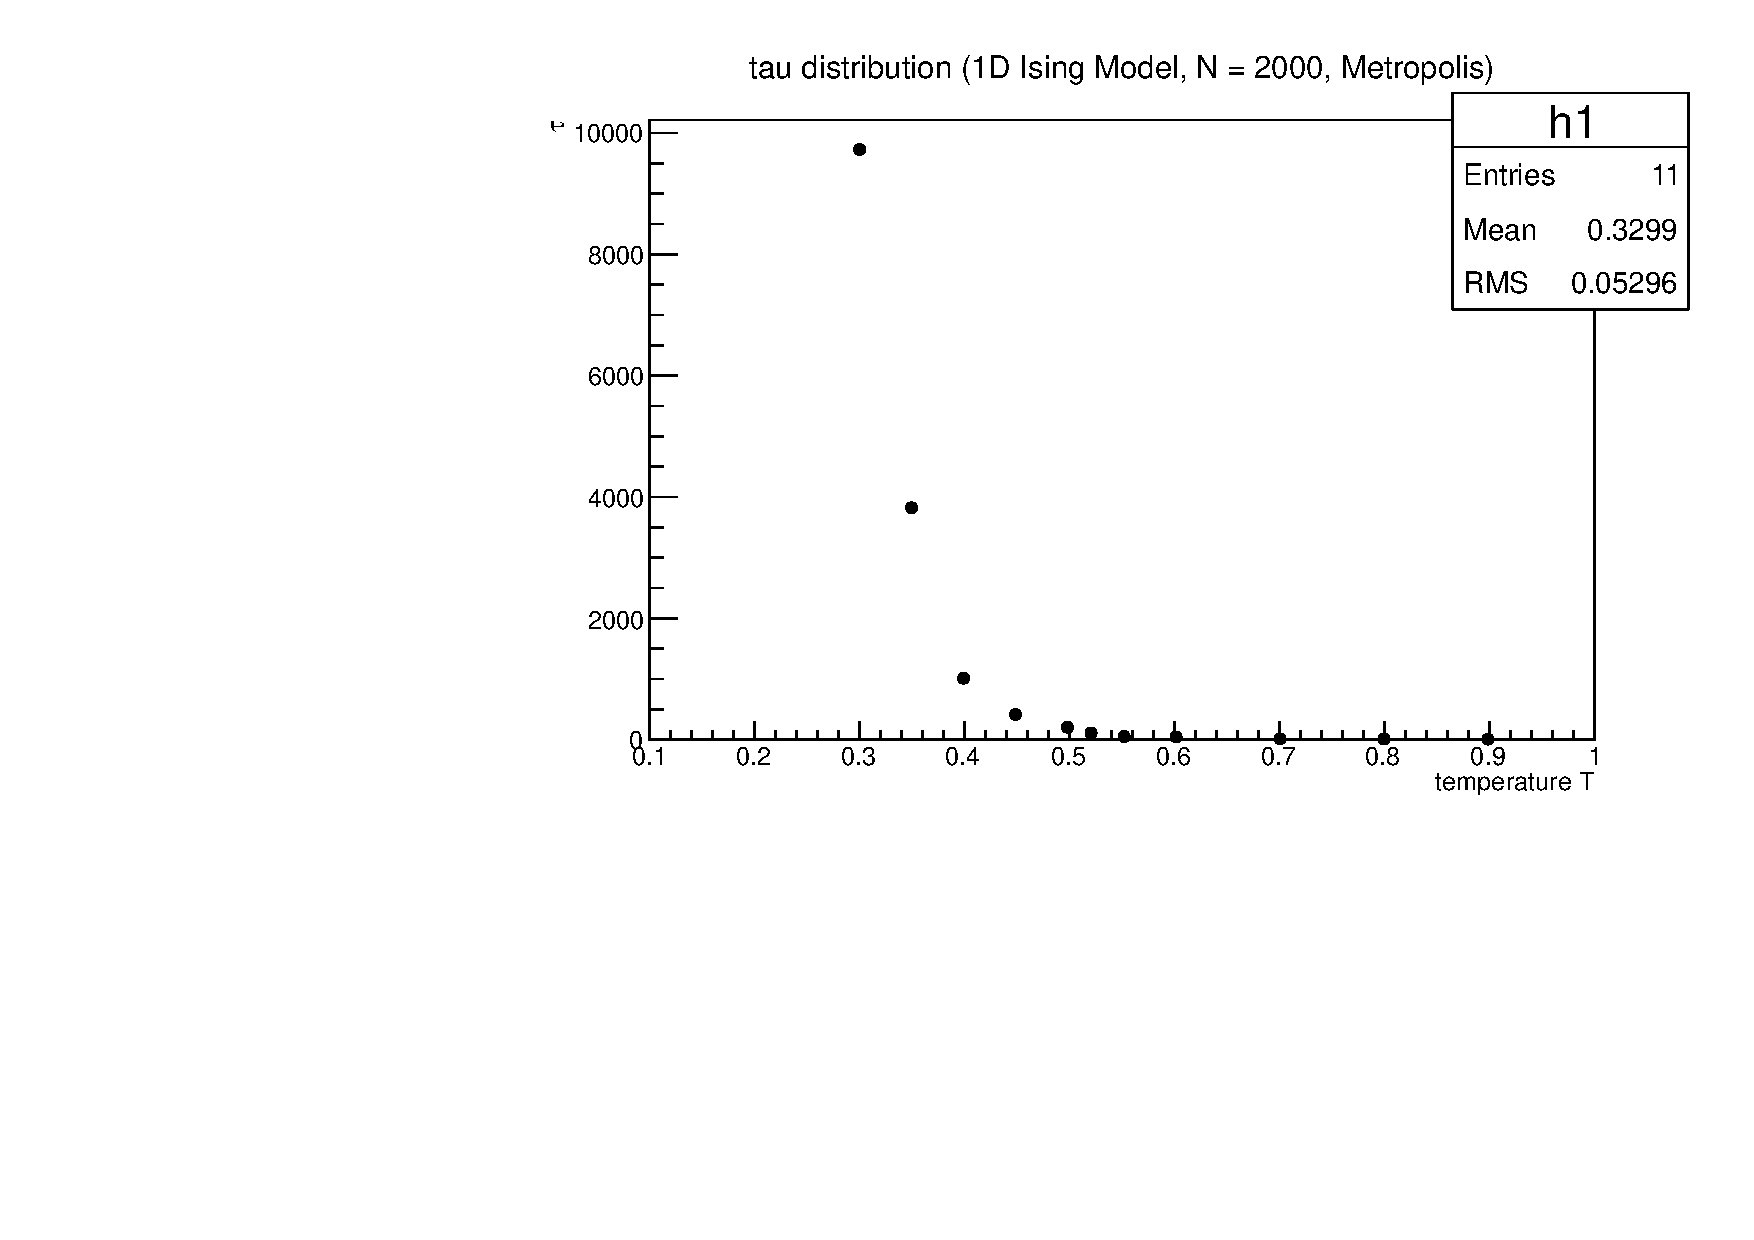
\includegraphics[scale=0.6]{IsingTestTCorr_T_vs_tau.pdf}
  \vspace{-0.05in}
   \caption[]{Correlation time $\tau$ as a function of temperature $T$ for 1D Ising model ($N=2000$) with Metropolis dynamics. Values of correlation times are found by fit analysis of the $\chi(t)$ function.}   
  \label{T_vs_tau_1d}
\end{figure}

\begin{figure}[!ht]
\centering
  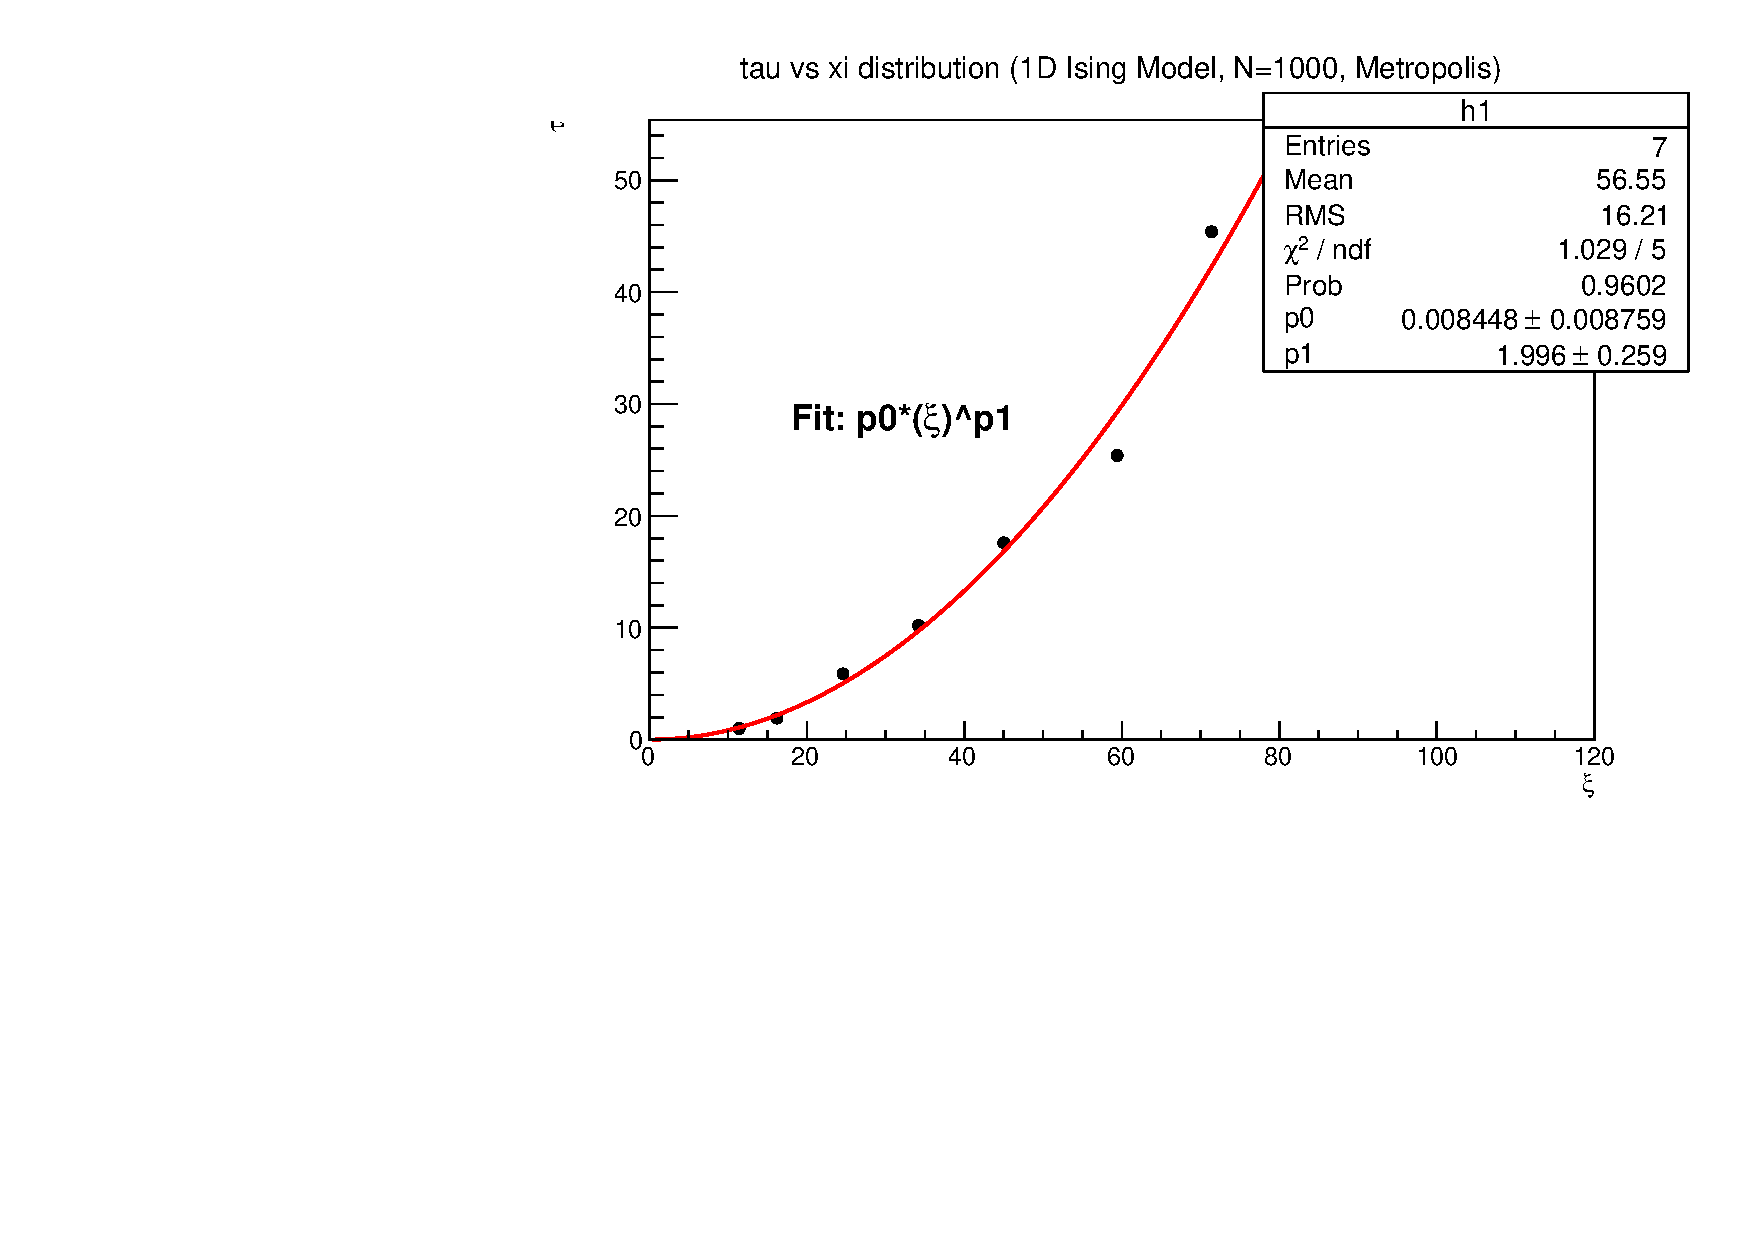
\includegraphics[scale=0.6]{tau_vs_xi.pdf}
  \vspace{-0.05in}
   \caption[]{Correlation time $\tau$ as a function of correlation length $\xi$ for 1D Ising model ($N=1000$) with Metropolis dynamics. Different points denote different temperatures: $T=1.2,~1.0,~0.8,~0.7, ~0.65,~0.6$ accordingly. Power function fit performed to get the dynamical exponent value is also shown.}   
  \label{tau_vs_xi_1d}
\end{figure}
 
\clearpage
\subsection{2D Ising model} 
Figure \ref{T_vs_tau_2d} presents the correlation time behaviour as a function of temperature for 2D Ising model ($N=16\times16$) with Metropolis dynamics. 
In this case, one can get the value of dynamical critical exponent of magnetization, using directly the relation (\ref{tauxi2}). To get the value of critical exponent $z$, a reduced power function fit is performed:
\begin{equation}
\tau(T)=a(T-T_c)^b ,
\end{equation}
with $T_c=2.15$.
 The power parameter from the fit gives the value of $-\nu z \approx -2.16$, which is in agreement with the expectations for 2D Ising model (where $\nu=1$).

\begin{figure}[!ht]
\centering
  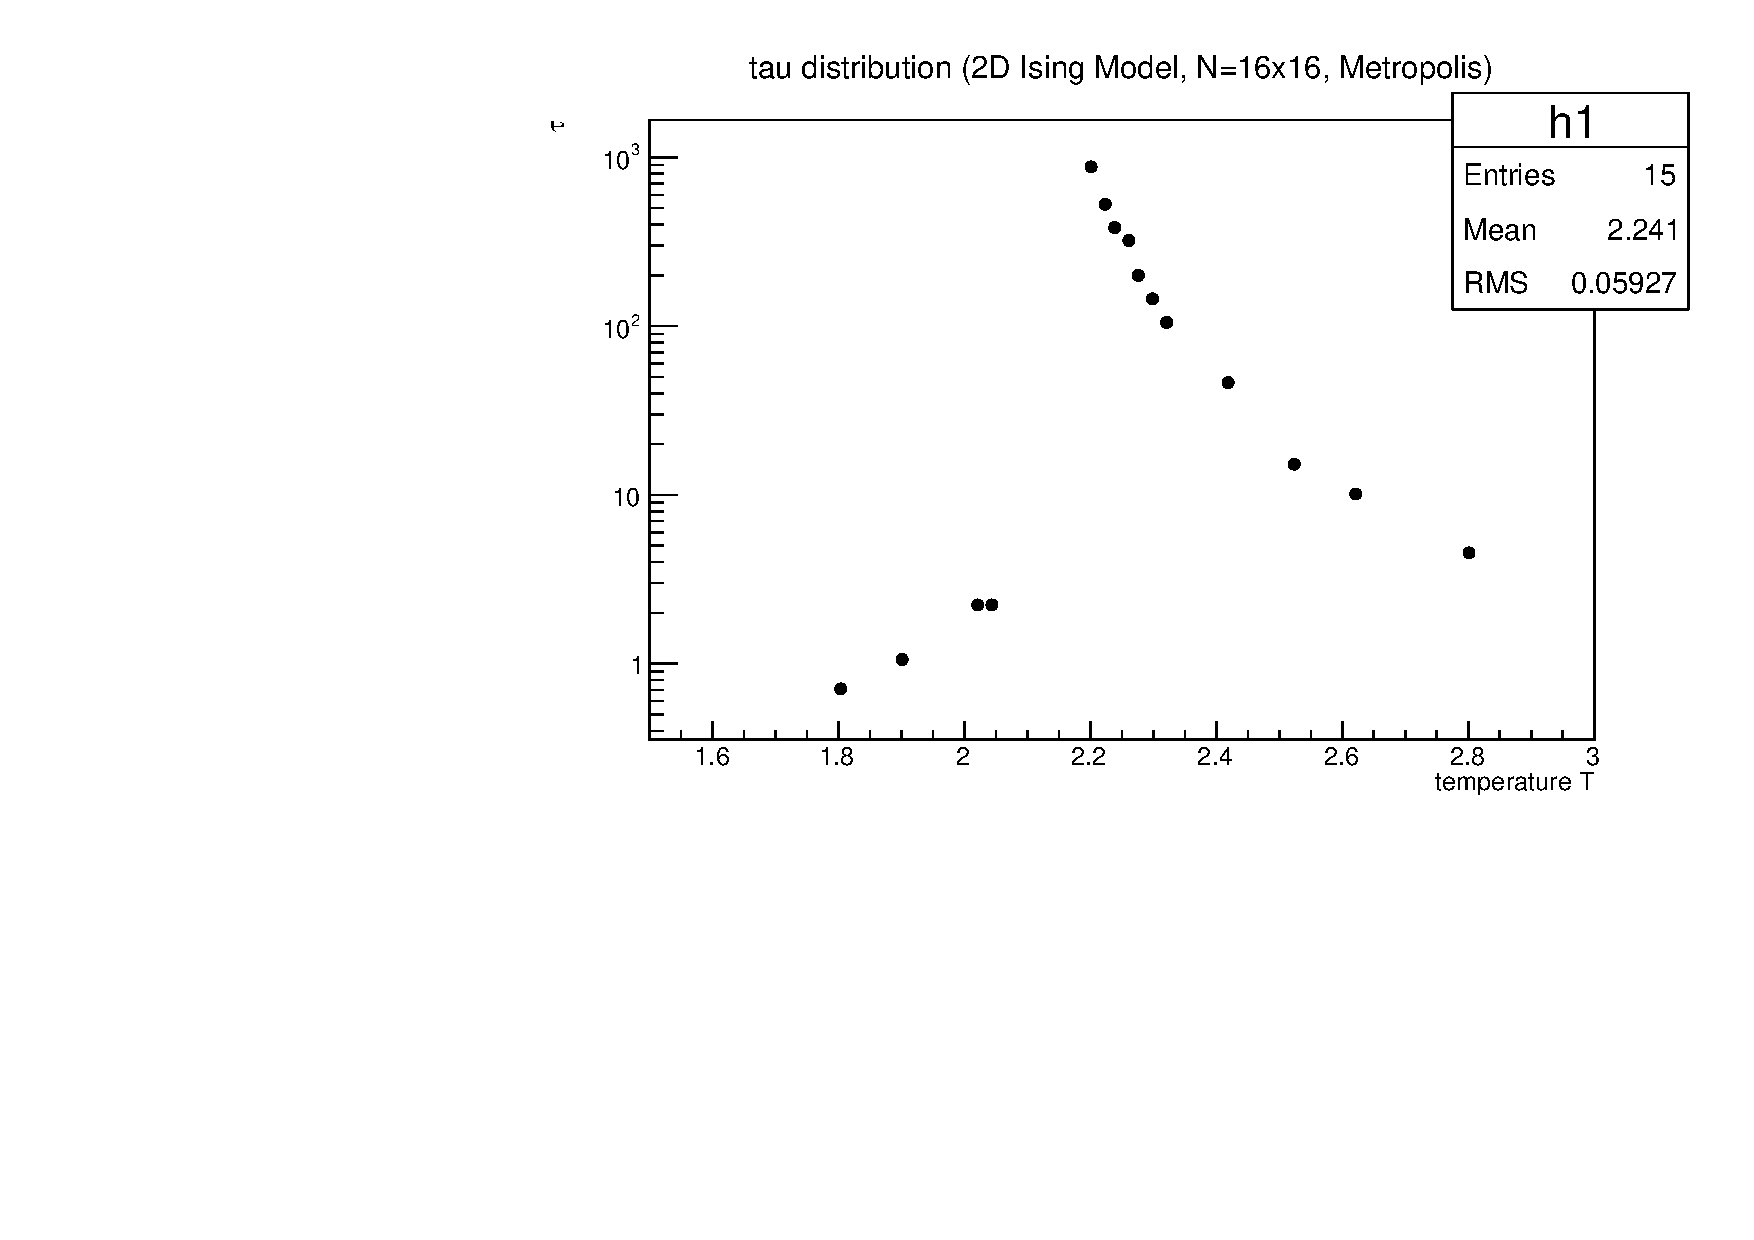
\includegraphics[scale=0.6]{IsingTestTCorr_T_vs_tau_log_2D.pdf}
  \vspace{-0.05in}
   \caption[]{Correlation time $\tau$ as a function of temperature $T$ for 2D Ising model ($N=16\times16$) with Metropolis dynamics. Values of correlation times are found by fit analysis of the $\chi(t)$ function.}   
  \label{T_vs_tau_2d}
\end{figure}

\begin{figure}[!ht]
\centering
  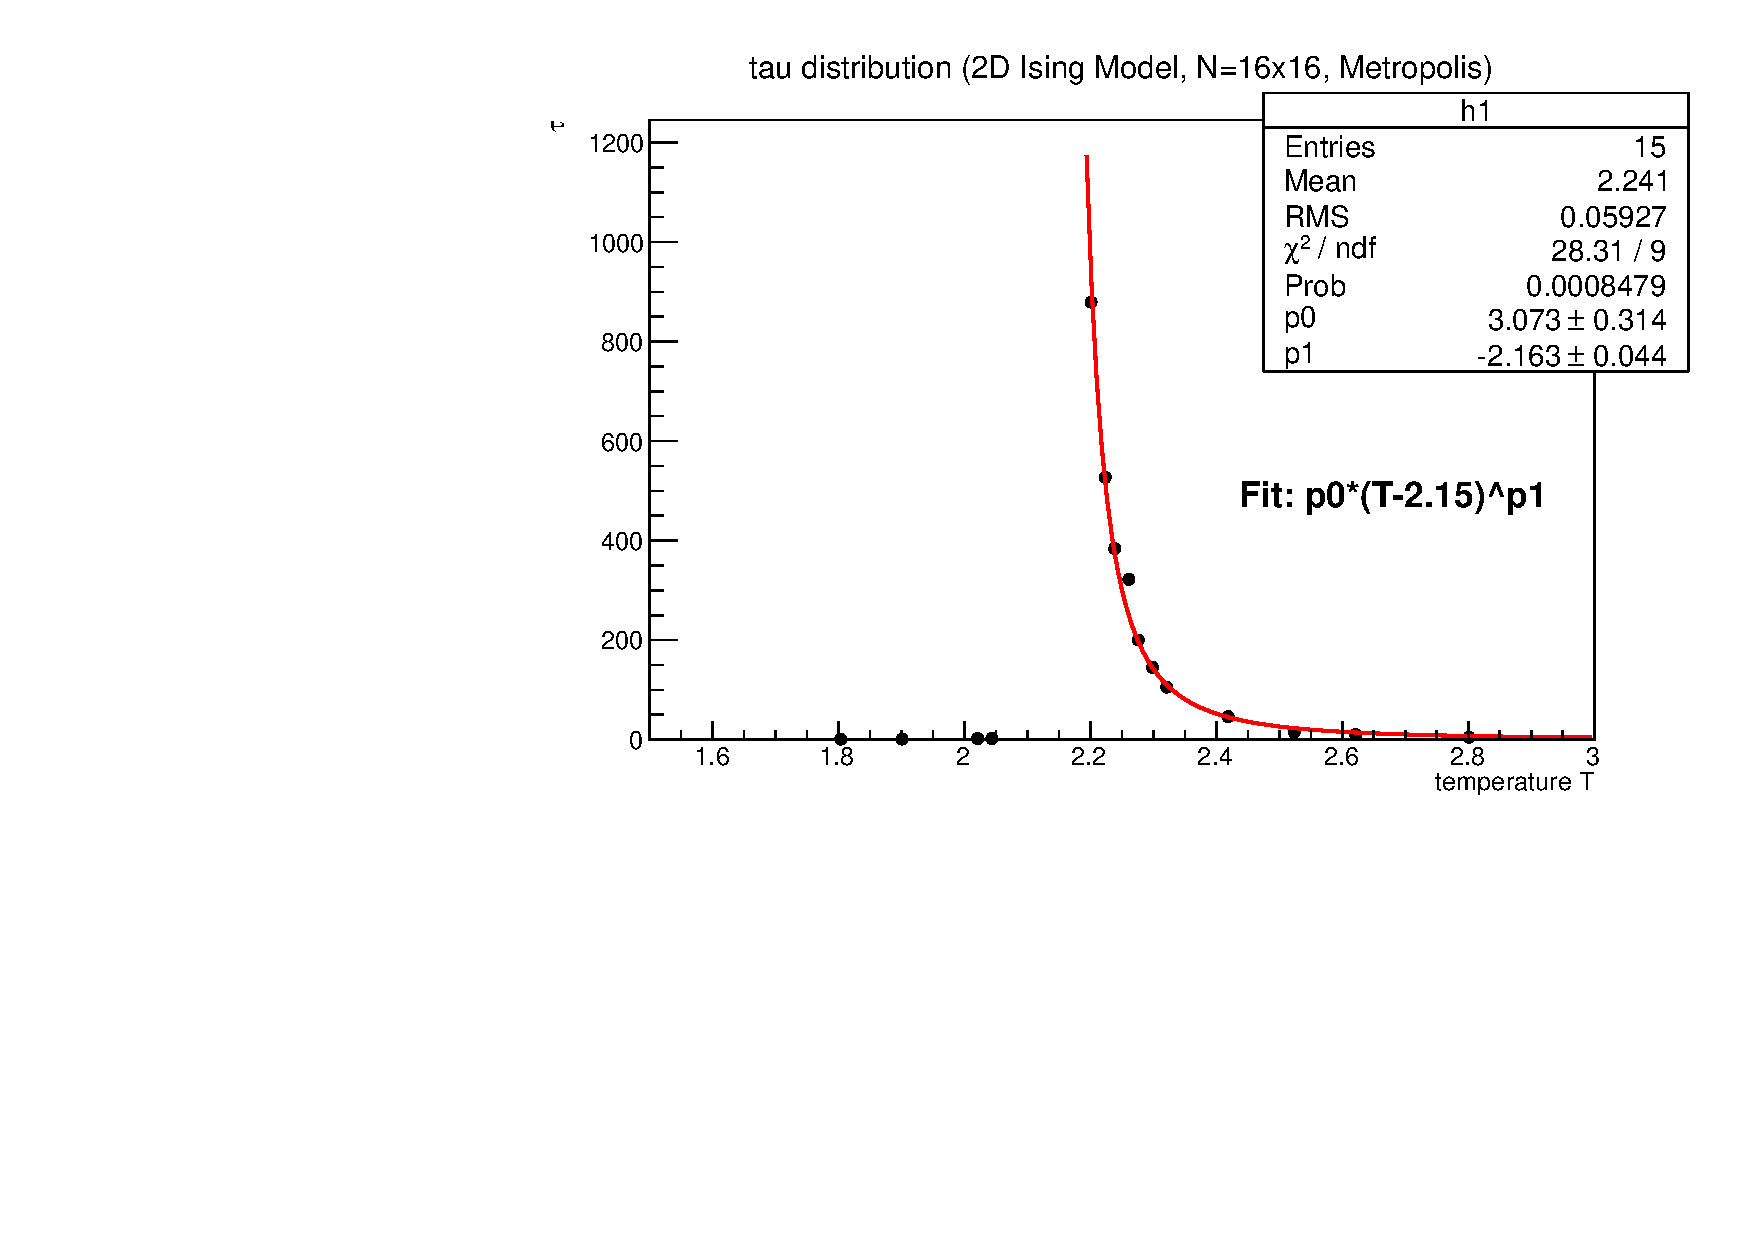
\includegraphics[scale=0.6]{IsingTestTCorr_T_vs_tau_fit_2D.pdf}
  \vspace{-0.05in}
   \caption[]{Fit procedure of correlation time $\tau$ as a function of temperature $T$ for 2D Ising model ($N=16\times16$) with Metropolis dynamics.  }   
  \label{tau_vs_xi_2d}
\end{figure}

\subsection{Wolff algorithm}
Figure \ref{gt_2d_wolff} presents an example of the autocorrelation function of magnetization for 2D Ising model with Wolff dynamics.
One can notice the correlation time value is below $1$. This trend is also observed for other temperatures, even for $T\approx T_c$.
This means that cluster algorithms almost eliminates critical slowing down effect.
%since one cluster flip in Wolff algorithm is not equivalent to one Monte Carlo step per spin in the Metropolis algorithm. 


\begin{figure}[!ht]
\centering
  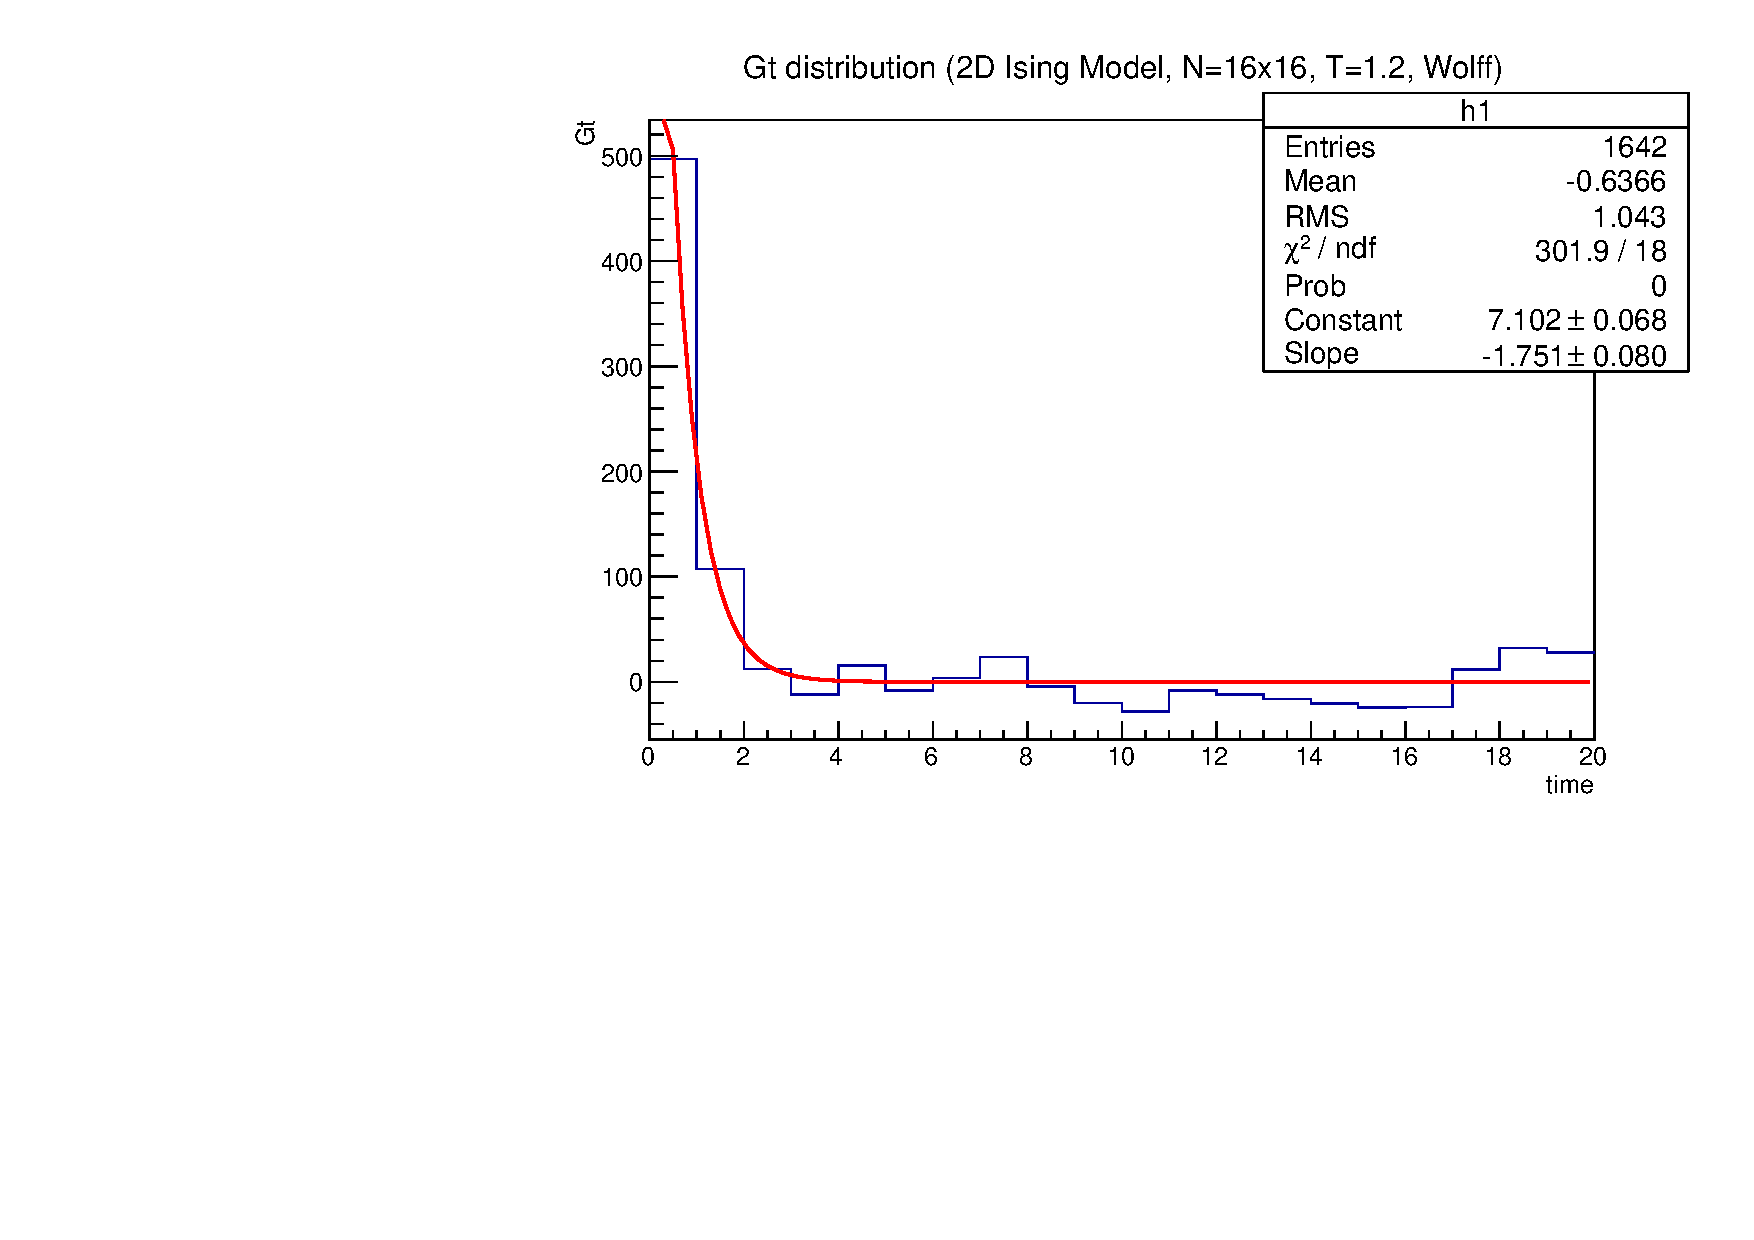
\includegraphics[scale=0.6]{Gt_2D_wolff.pdf}
  \vspace{-0.05in}
   \caption[]{Autocorrelation function (magnetization) for 2D Ising model with $N=16\times16$ lattice of spins and $T=1.2$. The value of the fit slope corresponds to $\tau=0.59$. Wolff algorithm is used in the simulation.}   
  \label{gt_2d_wolff}
\end{figure}

\clearpage
\section{Summary}
In this report basic properties of autocorrelation function for magnetization are presented. In particular, the relation between the function and correlation time.

The dynamical critical exponents for magnetization are estimated for 1D and 2D Ising models with Metropolis dynamics. They are in agreement with the theoretical value of $2$. This means that Metropolis algorithm is not very efficient when the system reaches critical point.

Finally, the dynamical properties of Wolff clustering algorithm are investigated: cluster algorithms almost eliminates critical slowing down effect.



%\clearpage
\bibliographystyle{unsrt}
\bibliography{common_project_mdyndal}







\end{document}
